%%%%%%%%%%%%%%%%%%%%%%%%%%%%%%%%%%%%%%%%%
% EPFL/Blue Brain Project
%
% Author:
% 	Quarta Jonny
%
% Date:
%	June 2014
%
%%%%%%%%%%%%%%%%%%%%%%%%%%%%%%%%%%%%%%%%%

%----------------------------------------------------------------------------------------
%	PACKAGES AND DOCUMENT CONFIGURATIONS
%----------------------------------------------------------------------------------------

\documentclass{article}


\usepackage{graphicx} % Required for the inclusion of images
\usepackage{multicol}
\usepackage[affil-it]{authblk}


\setlength\parindent{0pt} % Removes all indentation from paragraphs

\renewcommand{\labelenumi}{\alph{enumi}.} % Make numbering in the enumerate environment by letter rather than number (e.g. section 6)


%----------------------------------------------------------------------------------------
%	DOCUMENT INFORMATION
%----------------------------------------------------------------------------------------

\title{\textbf{Device Interface for motor/camera communication}} % Title

\author{Jonny \textsc{Quarta}} % Author name

\date{\today} % Date for the report
\affil{Ecole Polytechnique Federale de Lausanne}

\begin{document}

\maketitle % Insert the title, author and date

\tableofcontents

\section{Introduction}
The SpiNNaker is a very powerful device because it enables the user to run parallel simulations in a very efficient way. As already stated in other documents, it suffers however from various drawbacks, especially from the developer perspective. Indeed, when programming the device, the developer has very few debugging tools, the only one being the \textit{io\_printf} function, whose utilization is not advised because it alters the program behaviour. \\ \\

For these reasons an emulator has been created. The emulator also enables someone who does not have the SpiNNaker to program on it anyway.\\
In order to speed up the development time, one should first implement his program on the emulator, with the possibility of using all the available debugigng tools, and then port the code to the actual device.\\ \\

However, the emulator has some limitations, one of these being the fact that external devices (like motors or cameras) cannot be accessed. This is why a new emulator component has been designed.\\
\textbf{devin} (for DEVice INterface) is the component enabling the user to access the camera and the motors.\\
This document explores the way it has been constructed.

\section{Architecture}
Normally, there is no possibility to directly link the motors and the camera to a pc, even with the USB port. Or if there is, one needs to develop all the drivers to communicate with. \\
The proposed architecture takes advantage of the already existing links between the SpiNNaker and the peripherals.\\

The idea is to load a simple program into the SpiNNaker, whose purpose is to activate the motors and receive the camera input, as could do any normal loaded program. Finally, the pc emulator would communicate with the program on the SpiNNaker rather than directly with the peripherals. \\
This is achievable because the SpiNNaker provides a way to access the loaded program data.

\section{Communication Protocol}
In order to perform any operation from the pc to the SpiNNaker, UDP messages must be exchanged between the two devices. The Ethernet port of the SpiNNaker is actually always listening for incoming UDP packets. These packets contain SDP data (see the SpiNNaker official documentation for more details). Inside an SDP packet, SCP commands can be declared. These commands provide very low level operations, like reading or writing data at a particular memory address, or start executing from a certain location. Again, for more information, please consult the SpiNNaker documentation about SCP.\\

In order to communicate with the SpiNNaker, UDP packets must be sent to the good address. The SpiNNaker has IP address \textbf{192.168.0.11} and listens to the port \textbf{17893}. Therefore any UDP packets must be sent to this specific destination.\\

As already said, UDP packets must contain SDP data. The SDP information does follow a certain structure, which is depicted in figure \ref{fig:sdp}. The most important byte is the \textit{flags} one, which must be set to \textit{0x07} is no reply is expected or \textit{0x87} otherwise.
\begin{figure}[h]
\begin{center}
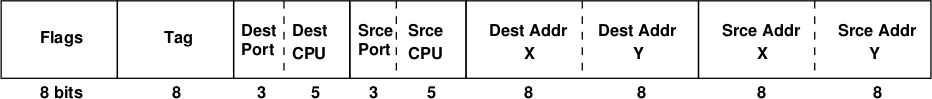
\includegraphics[width=0.9\textwidth]{sdp}
\caption{SDP packet structure}
\label{fig:sdp}
\end{center}
\end{figure}

After the SDP header, the UDP packet must contain SCP information, showed in figure \ref{fig:scp}. Here, \textit{cmd\_rc} must be set to \textit{0x02} for declaring a \textit{read} command and \textit{0x03} for a \textit{write} command. \textit{argX} corresponds to the arguments the specific command takes. In addition, it is possible to add extra data after the SCP header.
\begin{figure}[h]
\begin{center}
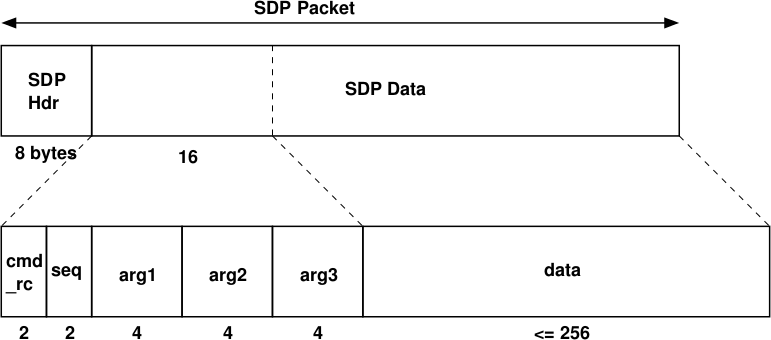
\includegraphics[width=0.9\textwidth]{scp}
\caption{SCP packet structure}
\label{fig:scp}
\end{center}
\end{figure}

Finally, figures \ref{fig:read} and \ref{fig:write} show the packet structure for the \textit{read} and \textit{write} commands. The \textit{Address} field indicate the memory location where to perform the operation, the \textit{Length} field declares the total number of bytes taken into account at that location and the \textit{Type} field must be set to \textit{0x02} for word values (4 bytes). Also note that the \textit{read} commands send a simple reply, as showed in figure \ref{fig:read}, which is also contained in a normal SDP packet.
\begin{figure}[h]
\begin{center}
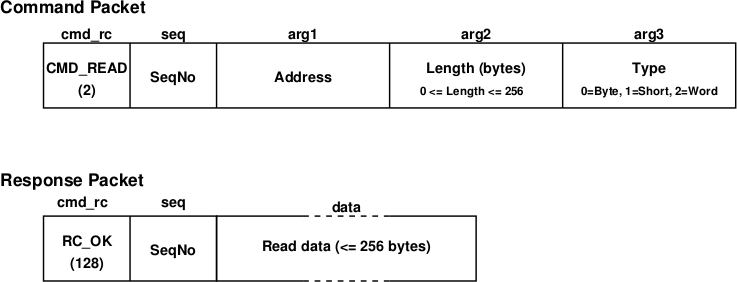
\includegraphics[width=0.9\textwidth]{read}
\caption{Read command structure}
\label{fig:read}
\end{center}
\end{figure}

\begin{figure}[h]
\begin{center}
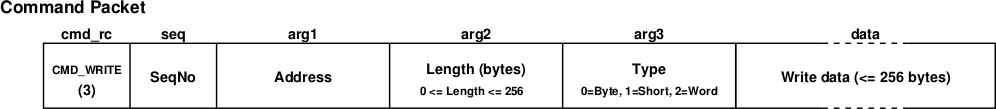
\includegraphics[width=0.9\textwidth]{write}
\caption{Write command structure}
\label{fig:write}
\end{center}
\end{figure}

\section{Emulator-side Implementation}
Once the protocol is set, this section deals with the actual implementation.\\

In order to access the \textbf{devin} features, the following header must be included into the project:
\begin{verbatim}
#include "spin_emu_devin.h"
\end{verbatim}
It contains the following functions:
\begin{verbatim}
int spin_devin_init()

unsigned int spin_devin_get_camera()

void spin_devin_send_motor(unsigned int command)

void spin_devin_dispose()
\end{verbatim}

In this section, the behaviour of these functions is explained.

\subsection{Initialization}
The \textit{spin\_devin\_init()} function initializes the connection to the SpiNNaker using the standard available C sockets. It performs the following actions:
\begin{verbatim}
// Declare new UDP socket, initialized to 0
spinn_id = socket(AF_INET, SOCK_DGRAM, IPPROTO_UDP);
memset((char *) &spinn_addr, 0, sizeof(spinn_addr));

// Set socket information (PORT is 17893 and ADDR is 192.168.0.11)
spinn_addr.sin_family = AF_INET;
spinn_addr.sin_port = htons(SPINNAKER_PORT);
inet_aton(SPINNAKER_ADDR, &spinn_addr.sin_addr);

// Returns 1 if everything fine, otherwise 0
return connected;
\end{verbatim}

This fucntion must be called by only one core at the beginning of every new emulator project.\\
The other function, \textit{spin\_devin\_dispose()}, releases the socket and must be called at the end of the simulation.

\subsection{Camera Input}
In order to obtain the next camera coordinate, the \textit{spin\_devin\_get\_camera()} function must be called. Note that this changes from the normal SpiNNaker behaviour, where one would rather wait for incoming events from the camera. Therefore, when porting the emulated code to the SpiNNaker, care must be taken about this.\\
The function performs the following actions:
\begin{verbatim}
- Declare buffers of size 26(cmd) and 18(reply), initialized to 0

- Set the following values into the command
buf[2] = 0x87; // reply expected
buf[3] = 0xff; // tag
buf[5] = 0xff; // source port/cpu
buf[10] = 0x2; // "read" command
buf[18] = 0x4; // length
buf[22] = 0x2; // type "word"

- Set the memory location where the camera
information is stored. Note that the SpiNNaker
memory follows the little endian convention,
therefore bytes have to be inverted.
Also note that the location is at address
0xF500003c, reserved to data (not program
code).
buf[14] = CAMERA_LOCATION & 0x000000ff;
buf[15] = (CAMERA_LOCATION >> 8) & 0x000000ff;
buf[16] = (CAMERA_LOCATION >> 16) & 0x000000ff;
buf[17] = (CAMERA_LOCATION >> 24) & 0x000000ff;

- Send the message and wait for reply

- Compute position from received data.
Note that the bytes have to be inverted
(little endian) and that this information
is stored from byte 14 in the response.
pos = (rcv_buf[17] << 24)|(rcv_buf[16] << 16 & 0x00ff0000)
 |(rcv_buf[15] << 8 & 0x0000ff00)|(rcv_buf[14] & 0x000000ff);

- Return camera position
return pos;
\end{verbatim}

\subsection{Motor Output}
The last important provided function enables the user to send motor commands. The structure follows the same of the camera operation:
\begin{verbatim}
- Declare buffer of size 34(cmd), initialized to 0

- Set the following values into the command
buf[2] = 0x07; // no reply expected
buf[3] = 0xff; // tag
buf[5] = 0xff; // source port/cpu
buf[10] = 0x3; // "write" command
buf[18] = 0x8; // length
buf[22] = 0x2; // type "word"

- Set the memory location where the motor
information will be read. Note that the SpiNNaker
memory follows the little endian convention,
therefore bytes have to be inverted.
Also note that the location is at address
0xF5000034, reserved to data (not program
code).
In addition, 2 words are actually sent,
located at contiguous addresses.
This is why the length is set to 8.
buf[14] = MOTOR_LOCATION & 0x000000ff;
buf[15] = (MOTOR_LOCATION >> 8) & 0x000000ff;
buf[16] = (MOTOR_LOCATION >> 16) & 0x000000ff;
buf[17] = (MOTOR_LOCATION >> 24) & 0x000000ff;

- Set the values. As already said, two words
are actually sent. The first one is the 
motor angles value (note the little endianness),
the other one is a byte used by the
program located on the SpiNNaker to check if
a new motor command has been provided.
// motor angles
buf[26] = command & 0x000000ff;
buf[27] = (command >> 8) & 0x000000ff;
buf[28] = (command >> 16) & 0x000000ff;
buf[29] = (command >> 24) & 0x000000ff;
// check value
buf[30] = 0x1;
buf[31] = 0x0; // same for buf[32] and buf[33]

- Send the message
\end{verbatim}

\section{SpiNNaker-side Implementation}
The last part of \textbf{devin} is the program loaded onto the SpiNNaker. Its behaviour is actually very simple. \\

The first step is to declare 3 pointers pointing to the locations of the camera, motor and check bytes. Then the program initializes the peripherals, as a normal SpiNNaker code would do. As a remainder, the code is the following:
\begin{verbatim}
#define EAST 0x1
#define CORE(n) (1<< (n+6))

#define MOTORS_KEY ((252 << 24) | (255 << 16))

#define MGMT_BIT 0x400
#define EVDS1_ENABLE 0x45

...
// Initialization

	// motor entry
	spin1_set_mc_table_entry(0x2, 	MOTORS_KEY, 0xFFFF0000,	EAST);

	spin1_set_mc_table_entry(0x1, 	EVDS1_ENABLE | MGMT_BIT, 
              0xFFFFFFFF, EAST);

	// camera reception entry
	spin1_set_mc_table_entry(0x3, 	0x0,	0x0, CORE(1));

	// activating camera
	spin1_send_mc_packet(EVDS1_ENABLE | MGMT_BIT, 1, 1);
\end{verbatim}

The last step is to take into account the information bytes.
\begin{verbatim}
void sendMotor(uint time, uint null){
    if(*check == 1) {
        spin1_send_mc_packet(MOTORS_KEY, *motor, 1);
        *check = 0;
    }
}

void cameraEvent(uint key, uint payload){
    *camera = key;
}
\end{verbatim}
Note that the motor event is called every 10ms and checks for an incoming motor command, in which case the motors are accessed.

\section{Conclusion}
The \textbf{devin} component works very well and is very responsive. Some simulations have been performed, showing that motor commands can be sent with a delay of 10ms between them without loosing performance.\\
In addition, ancien projects for the SpiNNaker were very easily ported to the simulator, giving the same results and performances as their counterpart.\\
\\
It is also notefully that, as pointed out by some developers, as the code loaded onto the SpiNNaker grows, more strange errors are encountered, which are certainly due to wrong memory overwritings by the hardware. The emulator does not suffer from these problems, enabling therefore correct program versions to be tested before ported to the SpiNNaker, thus avoiding spending a huge amount of time on strange bugs just because the SpiNNaker did not execute the code well. Of course, we wait for better SpiNNaker versions... 

\end{document}